\documentclass{article}
\usepackage{graphicx}
\usepackage{amsthm}
\usepackage{amssymb}
\usepackage{amsmath}
\usepackage{parskip}
\usepackage[margin=.85in]{geometry}
\usepackage{tikz}
\usepackage{titling}

 % move title upward

\title{15.C57 Optimization Methods HW1}
\author{Chris Low}
\date{} % removes the date

\begin{document}

\maketitle

\section*{Question 1}

\subsection*{(a)}
\textbf{True.}

Since $A$ has $m$ linearly independent rows, $\operatorname{rank}(A)=m$.
Since there are \(m\) independent equality constraints, they reduce the \(n\) variables to \(n-m\) degrees of freedom.
\[
n-\operatorname{rank}(A)=n-m=(m+1)-m=1.
\]
Thus, $Ax=b$ describes a line. Intersecting this line with our
nonnegativity constraints $x\geq 0$ gives us a feasible region with at most
two extreme points. Since basic feasible solutions correspond to extreme
points, $\mathcal{P}$ has at most two basic feasible solutions. \qed 



\vspace{5mm}
\subsection*{(b)}

\textbf{False.}
A basic feasible solution can have at most $m$ positive variables, but an optimal solution does not have to be a basic feasible solution; it may lie between extreme points when there are multiple optimal solutions.

Consider an example with $m=2$ constraints and $n=3$ variables:
\[
x_1+x_2+x_3=3,
\]
\[
x_1-x_2=0,
\]
with
\[
x_1,x_2,x_3\geq 0.
\]

Let
\[
c=(0,0,0)^\top.
\]
This makes our objective
\[
\min c^\top x
=
\min (0x_1+0x_2+0x_3)
=
0.
\]
Therefore, every feasible solution is optimal.

For example, 
\[
x=(1,1,1)^\top
\]
is feasible and optimal. However, all three variables are positive, while
$m=2$. Thus, this optimal solution has more than $m$ positive variables,
so the statement is false.

\vspace{5mm}

\subsection*{(c)}

\textbf{True.}

If the linear optimization problem has an optimal solution, then there
exists an optimal solution $x^*$ that is an extreme point of $\mathcal{P}$.
Since extreme points are equivalent to basic feasible solutions, $x^*$ is
also a basic feasible solution.

For a standard-form polyhedron, a basic feasible solution has $n-m$
nonbasic variables set to zero. Therefore, at most $m$ variables can be
positive. Hence, there exists an optimal solution with at most $m$ positive
variables.


\vspace{5mm}

\subsection*{(d)}
\textbf{True.}

By the theorem from L2 slide 11, a point is a basic feasible solution if and only if it is an extreme point of $\mathcal{P}$. Thus, $x$ and $y$ are
two distinct extreme points of $\mathcal{P}$.

For any $\lambda \in (0,1)$, let
\[
z=\lambda x+(1-\lambda)y.
\]
Since $0<\lambda<1$ and $x\neq y$, the point $z$ lies between the two
distinct feasible points $x$ and $y$. By the definition of an extreme
point, $z$ cannot be an extreme point of $\mathcal{P}$.

Therefore, by the equivalence between extreme points and basic feasible
solutions, $z$ is not a basic feasible solution.





\vspace{5mm}
\subsection*{(e)}

\textbf{True.}

Let $x_j$ be a nonbasic variable with zero reduced cost,
\[
\bar c_j=0.
\]

Since $x$ is nondegenerate, all basic variables are strictly positive.
Therefore, for the direction $d$ associated with increasing $x_j$, we can
choose a sufficiently small $\theta>0$ such that
\[
y=x+\theta d
\]
is still feasible. Since $\theta>0$, we have $y\neq x$.

The objective value at $y$ is
\[
c^\top y
= c^\top(x+\theta d)
= c^\top x+\theta \bar c_j
= c^\top x.
\]

Thus, $y$ has the same objective value as $x$. Since $x$ is optimal,
$y$ is also optimal. Therefore, there are at least two distinct optimal
solutions, so $x$ is not the unique optimal solution.



\vspace{5mm}
\subsection*{(f)}
\textbf{False.}

The function $\max\{c^\top x,d^\top x\}$ is convex, since it is the
maximum of two linear functions, but it is not necessarily linear.
Therefore, the theorem that a linear optimization problem has an optimal
solution at an extreme point does not necessarily apply.

Consider the one-dimensional polyhedron
\[
\mathcal P=[-1,1].
\]
Its extreme points are $-1$ and $1$.

Let
\[
c=1
\qquad\text{and}\qquad
d=-1.
\]

\[
c^\top x=x
\qquad\text{and}\qquad
d^\top x=-x.
\]
Therefore, our objective becomes
\[
\max\{c^\top x,d^\top x\}
=
\max\{x,-x\}
=
|x|.
\]

Hence, our problem to minimize is
\[
\min_{x\in[-1,1]} |x|.
\]
The minimum is attained at
\[
x^*=0,
\]
with objective value $0$.

However, $0$ is not an extreme point of $\mathcal P$, since it lies
between the two extreme points $-1$ and $1$. At either extreme point,
the objective value is $1$.

Thus, the problem has an optimal solution, but no optimal solution is an
extreme point of $\mathcal P$. Therefore, the statement is false.


\newpage




\section*{Question 2}

The feasible region is determined by
\[
x_1+x_2\leq 5,
\]
\[
2x_1+x_2\leq 8,
\]
\[
x_1+3x_2\leq 9,
\]
together with \(x_1,x_2\geq 0\).

\subsection*{(a)}



We first find the extreme points on the coordinate axes. Setting \(x_2=0\), the constraints imply
\[
x_1\leq 5,\qquad x_1\leq 4,\qquad x_1\leq 9,
\]
so the extreme point on the \(x_1\)-axis is
\[
\boxed{(4,0).}
\]

Similarly, setting \(x_1=0\), the constraints imply
\[
x_2\leq 5,\qquad x_2\leq 8,\qquad x_2\leq 3,
\]
so the extreme point on the \(x_2\)-axis is
\[
\boxed{(0,3).}
\]

To find the remaining extreme point, consider the intersection of the first two constraints:
\[
x_1+x_2=5,
\]
\[
2x_1+x_2=8.
\]
Subtracting the first equation from the second gives us 
\[
x_1=3, \quad x_2=2.  \quad
    \boxed{(3,2).}
\]

\[
3+3(2)=9,
\]
So the third constraint is also active at this point.

We summarize: 
\[
\begin{array}{c|c}
\text{Extreme point} & \text{Active inequality constraints}\\
\hline
(0,0) & \text{None}\\
(4,0) & 2x_1+x_2=8\\
(3,2) & x_1+x_2=5,\; 2x_1+x_2=8,\; x_1+3x_2=9\\
(0,3) & x_1+3x_2=9
\end{array}
\]

The feasible region has extreme points
\[
\boxed{(0,0),\qquad (4,0),\qquad (3,2),\qquad (0,3).}
\]


\begin{center}
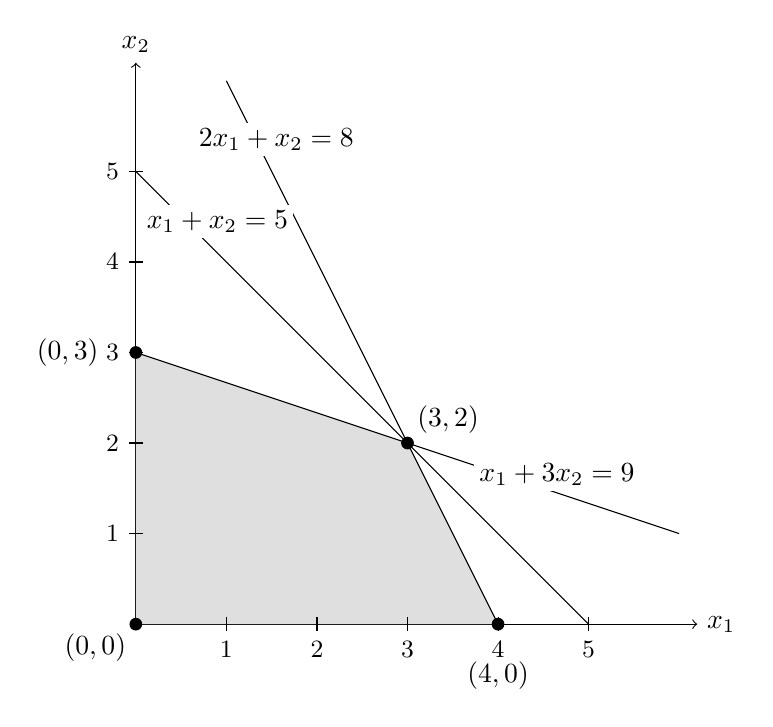
\begin{tikzpicture}[scale=1.15]

% Axes
\draw[->] (0,0) -- (6.2,0) node[right] {$x_1$};
\draw[->] (0,0) -- (0,6.2) node[above] {$x_2$};

% Feasible region
\fill[gray!25]
    (0,0) -- (4,0) -- (3,2) -- (0,3) -- cycle;

% Constraint lines
\draw (0,5) -- (5,0);
\draw (1,6) -- (4,0);
\draw (0,3) -- (6,1);

% Constraint labels -- manually positioned to avoid overlap
\node[fill=white, inner sep=2pt] at (0.9,4.45)
    {$x_1+x_2=5$};

\node[fill=white, inner sep=2pt] at (1.55,5.35)
    {$2x_1+x_2=8$};

\node[fill=white, inner sep=2pt] at (4.65,1.65)
    {$x_1+3x_2=9$};

% Extreme points
\fill (0,0) circle (2pt)
    node[below left] {$(0,0)$};

\fill (4,0) circle (2pt)
    node[below=10pt] {$(4,0)$};

\fill (3,2) circle (2pt)
    node[above right] {$(3,2)$};

\fill (0,3) circle (2pt)
    node[left=10pt] {$(0,3)$};

% Tick marks on x-axis
\foreach \x in {1,2,3,4,5}
    \draw (\x,0.08) -- (\x,-0.08)
    node[below] {\small \x};

% Tick marks on y-axis
\foreach \y in {1,2,3,4,5}
    \draw (0.08,\y) -- (-0.08,\y)
    node[left] {\small \y};

\end{tikzpicture}
\end{center}






\vspace{5mm}
\subsection*{(b)}


We rewrite with slack variables $s_1,s_2,s_3 \geq 0$, so the problem in
standard form is
\[
\max \quad x_1+\lambda x_2
\]
subject to
\[
x_1+x_2+s_1=5,
\]
\[
2x_1+x_2+s_2=8,
\]
\[
x_1+3x_2+s_3=9,
\]
\[
x_1,x_2,s_1,s_2,s_3\geq 0.
\]

There are three equality constraints, so each basis contains three
variables. For each extreme point, the corresponding slack variables
and one possible basis are:

\[
\begin{array}{c|c|c}
(x_1,x_2) &
(x_1,x_2,s_1,s_2,s_3) &
\text{One basis} \\
\hline
(0,0) & (0,0,5,8,9) & \{s_1,s_2,s_3\} \\
(4,0) & (4,0,1,0,5) & \{x_1,s_1,s_3\} \\
(0,3) & (0,3,2,5,0) & \{x_2,s_1,s_2\} \\
(3,2) & (3,2,0,0,0) & \{x_1,x_2,s_1\}
\end{array}
\]

The BFS corresponding to $(3,2)$ is degenerate. Since there are
three equality constraints, a basis must contain three variables.
However, at $(3,2)$,
\[
s_1=s_2=s_3=0.
\]
So any basis corresponding to this point must contain a
zero-valued basic variable. For example, with basis
\[
\{x_1,x_2,s_1\},
\]
the basic variables have values
\[
(x_1,x_2,s_1)=(3,2,0).
\]
Therefore, this BFS is degenerate.

The other three BFSs are nondegenerate since all basic variables in
the displayed bases are strictly positive.

Geometrically, $(3,2)$ is degenerate because all three inequality
constraints are active at this point:
\[
x_1+x_2=5,\qquad
2x_1+x_2=8,\qquad
x_1+3x_2=9.
\]
Since the problem is two-dimensional, only two linearly independent
active constraints are needed to determine an extreme point. As we have
three active constraints at $(3,2)$, this corresponds to degeneracy.





\vspace{5mm}

\subsection*{(c)}

The objective function is
\[
x_1+\lambda x_2.
\]

At each extreme point, we see: 
\[
\begin{array}{c|c}
\text{Extreme point} & \text{Objective value}\\
\hline
(0,0) & 0\\
(4,0) & 4\\
(3,2) & 3+2\lambda\\
(0,3) & 3\lambda
\end{array}
\]

The origin will never "win" because $(4,0)$ always gives $4 > 0$. We first compare $(4,0)$ and
$(3,2)$:
\[
4=3+2\lambda, \quad 
\lambda=\frac12.
\]

Next, compare $(3,2)$ and $(0,3)$:
\[
3+2\lambda=3\lambda, \quad
\lambda=3.
\]

We can see that for values of $\lambda$ away from these breakpoints,
\[
\boxed{x^*(\lambda)=
\begin{cases}
(4,0), & \lambda<\frac12,\\[2mm]
(3,2), & \frac12<\lambda<3,\\[2mm]
(0,3), & \lambda>3.
\end{cases}}
\]

We also observe that multiple optima occur at $\lambda = \frac{1}{2}$ and $\lambda = 3$. 


At $\lambda=\frac12$, the objective becomes
\[
x_1+\frac12x_2.
\]
Dividing constraint (2) by $2$ gives
\[
x_1+\frac12x_2\leq 4.
\]
So the objective value is at most $4$, and every feasible point
satisfying
\[
2x_1+x_2=8
\]
attains this value.


Therefore, the entire feasible edge from $(4,0)$
to $(3,2)$ is optimal. Hence the complete set of optimal solutions is
the line segment joining $(4,0)$ and $(3,2)$:
\[
\boxed{
\left\{
t(4,0)+(1-t)(3,2):0\le t\le1
\right\}.}
\]

At $\lambda=3$, the objective is
\[
x_1+3x_2.
\]
Since
\[
x_1+3x_2\le9,
\]
every point on the feasible edge
\[
x_1+3x_2=9
\]
has objective value $9$. So we get our complete set of optimal solutions, which is the line segment joining $(3,2)$ and $(0,3)$:
\[
\boxed{
\left\{
t(3,2)+(1-t)(0,3):0\le t\le1
\right\}.}
\]

Thus,
\[
\boxed{
\operatorname{argmax}=
\begin{cases}
\{(4,0)\}, & \lambda<\frac12,\\[1mm]
[(4,0),(3,2)], & \lambda=\frac12,\\[1mm]
\{(3,2)\}, & \frac12<\lambda<3,\\[1mm]
[(3,2),(0,3)], & \lambda=3,\\[1mm]
\{(0,3)\}, & \lambda>3.
\end{cases}}
\]

The problem has multiple optimal solutions precisely when
\[
\boxed{\lambda=\frac12 \quad\text{or}\quad \lambda=3.}
\]





\vspace{5mm}
\subsection*{(d)}

For $\lambda=1$, the problem in standard form is
\[
\max \quad x_1+x_2
\]
subject to
\[
x_1+x_2+s_1=5,
\]
\[
2x_1+x_2+s_2=8,
\]
\[
x_1+3x_2+s_3=9,
\]
\[
x_1,x_2,s_1,s_2,s_3\geq 0.
\]

We use: 
\[
(x_1,x_2,s_1,s_2,s_3),
\]
we have
\[
A=
\begin{pmatrix}
1&1&1&0&0\\
2&1&0&1&0\\
1&3&0&0&1
\end{pmatrix},
\qquad
b=
\begin{pmatrix}
5\\
8\\
9
\end{pmatrix},
\qquad
c=
\begin{pmatrix}
1\\
1\\
0\\
0\\
0
\end{pmatrix}.
\]

For this maximization problem, we use the reduced costs
\[
\bar c^\top
=
c^\top-c_B^\top B^{-1}A.
\]
A positive reduced cost indicates an improving direction.


\newpage
\textbf{Initial BFS.}

Starting with $x_1=x_2=0$ gives us 
\[
(x_1,x_2,s_1,s_2,s_3)=(0,0,5,8,9).
\]

The initial basis is
\[
\{s_1,s_2,s_3\},
\]
so
\[
B=I,
\qquad
B^{-1}=I,
\qquad
c_B=
\begin{pmatrix}
0\\
0\\
0
\end{pmatrix}.
\]

Therefore,
\[
\bar c^\top
=
c^\top-c_B^\top B^{-1}A
=
\begin{pmatrix}
1&1&0&0&0
\end{pmatrix}.
\]

Both $x_1$ and $x_2$ have positive reduced cost. We choose $x_1$ to
enter the basis.

The entering column is
\[
A_1=
\begin{pmatrix}
1\\
2\\
1
\end{pmatrix}.
\]

The direction of the basic variables is
\[
d_B=-B^{-1}A_1
=
\begin{pmatrix}
-1\\
-2\\
-1
\end{pmatrix}.
\]

Thus,
\[
s_1=5-\theta,
\qquad
s_2=8-2\theta,
\qquad
s_3=9-\theta.
\]

The minimum-ratio test gives us 
\[
\theta^*
=
\min\left\{
\frac{5}{1},
\frac{8}{2},
\frac{9}{1}
\right\}
=4.
\]

Therefore, we let $s_2$ leaves the basis and the new BFS is
\[
(x_1,x_2,s_1,s_2,s_3)
=
(4,0,1,0,5).
\]

\textbf{Second iteration.}

The new basis is
\[
\{s_1,x_1,s_3\}.
\]

Thus,
\[
B=
\begin{pmatrix}
1&1&0\\
0&2&0\\
0&1&1
\end{pmatrix},
\]

\[
B^{-1}
=
\begin{pmatrix}
1&-\frac12&0\\
0&\frac12&0\\
0&-\frac12&1
\end{pmatrix}.
\]

Since the basic variables are $(s_1,x_1,s_3)$,
\[
c_B=
\begin{pmatrix}
0\\
1\\
0
\end{pmatrix}.
\]


\[
c_B^\top B^{-1}
=
\begin{pmatrix}
0&\frac12&0
\end{pmatrix},
\]

\[
c_B^\top B^{-1}A
=
\begin{pmatrix}
1&\frac12&0&\frac12&0
\end{pmatrix}.
\]

\[
\bar c^\top
=
\begin{pmatrix}
1&1&0&0&0
\end{pmatrix}
-
\begin{pmatrix}
1&\frac12&0&\frac12&0
\end{pmatrix}
=
\begin{pmatrix}
0&\frac12&0&-\frac12&0
\end{pmatrix}.
\]

Since
\[
\bar c_{x_2}=\frac12>0,
\]
$x_2$ enters the basis.

The entering column is
\[
A_2=
\begin{pmatrix}
1\\
1\\
3
\end{pmatrix}.
\]

The direction of the basic variables is
\[
d_B=-B^{-1}A_2
=
-
\begin{pmatrix}
1&-\frac12&0\\
0&\frac12&0\\
0&-\frac12&1
\end{pmatrix}
\begin{pmatrix}
1\\
1\\
3
\end{pmatrix}
=
\begin{pmatrix}
-\frac12\\
-\frac12\\
-\frac52
\end{pmatrix}.
\]

Since the basic variables are ordered as $(s_1,x_1,s_3)$, we have
\[
s_1=1-\frac12\theta,
\]
\[
x_1=4-\frac12\theta,
\]
\[
s_3=5-\frac52\theta.
\]

The minimum-ratio test gives
\[
\theta^*
=
\min\left\{
\frac{1}{1/2},
\frac{4}{1/2},
\frac{5}{5/2}
\right\}
=
\min\{2,8,2\}
=2.
\]

There is a tie between $s_1$ and $s_3$. Choose $s_1$ to leave the
basis. At $\theta=2$, the new BFS is
\[
(x_1,x_2,s_1,s_2,s_3)
=
(3,2,0,0,0).
\]



With $s_1$ leaving and $x_2$ entering, choose the basis
\[
\{x_2,x_1,s_3\}.
\]


\[
B=
\begin{pmatrix}
1&1&0\\
1&2&0\\
3&1&1
\end{pmatrix},
\]

\[
B^{-1}
=
\begin{pmatrix}
2&-1&0\\
-1&1&0\\
-5&2&1
\end{pmatrix}.
\]


\[
c_B=
\begin{pmatrix}
1\\
1\\
0
\end{pmatrix}.
\]


\[
c_B^\top B^{-1}
=
\begin{pmatrix}
1&0&0
\end{pmatrix},
\]

\[
c_B^\top B^{-1}A
=
\begin{pmatrix}
1&1&1&0&0
\end{pmatrix}.
\]


\[
\bar c^\top
=
\begin{pmatrix}
1&1&0&0&0
\end{pmatrix}
-
\begin{pmatrix}
1&1&1&0&0
\end{pmatrix}
=
\begin{pmatrix}
0&0&-1&0&0
\end{pmatrix}.
\]

The nonbasic variables are $s_1$ and $s_2$, with
\[
\bar c_{s_1}=-1,
\qquad
\bar c_{s_2}=0.
\]

Since all nonbasic reduced costs are nonpositive, there is no
improving direction. Therefore the current BFS is optimal.


\[
\boxed{x_1^*=3,
\qquad
x_2^*=2,}
\]
with optimal objective value
\[
z^*=3+2=5.
\]

The simplex iterations we get: 
\[
\boxed{
(0,0,5,8,9)
\longrightarrow
(4,0,1,0,5)
\longrightarrow
(3,2,0,0,0).}
\]

First iteration: $x_1$ enters, $s_2$ leaves, and
$\theta^*=4$. 

Second iteration: $x_2$ enters, there is a tie
between $s_1$ and $s_3$ for the leaving variable, and
$\theta^*=2$. We choose $s_1$ to leave which yields the optimal BFS above.







\vspace{5mm}

\subsection*{(e)}


In the second ratio test, both $s_1$ and $s_3$ become zero at
\[
\theta=2.
\]
This means that two constraints become tight at the same time when we reach
\[
(x_1,x_2)=(3,2).
\]

Since only one variable leaves the basis, the other one stays basic with value zero. Therefore, the new BFS is \textbf{degenerate}.

However, this does not mean that simplex fails to make progress. In this step, we have
\[
\theta=2>0,
\]
and the objective value increases from $4$ to $5$. Thus, we still move to a better solution.

Degeneracy can cause a later pivot to have $\theta=0$. In our case, after reaching $(3,2)$, one of the basic variables, $s_3$, is already equal to zero. If a later pivot requires $s_3$ to decrease, the ratio test would give $\theta=0$ since $s_3$ cannot become negative. The basis could then change without changing the actual solution or objective value. However, this does not happen in the iteration above, since we reach $(3,2)$ with a positive step size $\theta=2$ and the objective increases from $4$ to $5$.



\section*{Question 3}

\vspace{5mm}
\subsection*{(a)}
Let
\[
B = [A_{B(1)},\ldots,A_{B(m)}]
\]
be the matrix formed by the $m$ basic columns of $A$. By assumption,
these columns are linearly independent. Since $B$ is an $m\times m$
matrix, it follows that $B$ is invertible.

There are $n-m$ nonbasic variables. We partition these variables into
the sets $L$ and $U$, and fix them at their bounds:
\[
x_j = 0 \qquad \text{for } j\in L,
\]
and
\[
x_j = u_j \qquad \text{for } j\in U.
\]
Therefore, each of the $n-m$ nonbasic variables has an active bound
constraint.

We now consider the equality constraints
\[
Ax=b.
\]
When we separate the basic and nonbasic variables, we get
\[
Bx_B
+
\sum_{j\in L} A_j x_j
+
\sum_{j\in U} A_j x_j
=
b.
\]
Since $x_j=0$ for $j\in L$ and $x_j=u_j$ for $j\in U$, this becomes
\[
Bx_B+\sum_{j\in U}A_j u_j=b.
\]


\[
Bx_B
=
b-\sum_{j\in U}A_j u_j.
\]
Since $B$ is invertible, we can solve uniquely for the basic variables:
\[
x_B
=
B^{-1}
\left(
b-\sum_{j\in U}A_j u_j
\right).
\]

Hence, the $n-m$ active bound constraints uniquely determine all of the
nonbasic variables, while the $m$ equality constraints uniquely determine
the remaining $m$ basic variables. Therefore, all $n$ variables are
uniquely determined by these active constraints.

In other words, these active constraints have full rank $n$. By the
definition of a basic solution (active constraints span the whole space), the resulting vector $x$ is therefore
a basic solution. \qed


\vspace{5mm}


For the nondegeneracy condition, recall that the $n-m$ nonbasic
variables are fixed at either their lower or upper bounds. Thus, their
$n-m$ bound constraints are active. Together with the $m$ equality
constraints $Ax=b$, these give the $n$ active constraints defining the
basic solution.

Suppose first that every basic variable satisfies
\[
x_j \neq 0
\qquad\text{and}\qquad
x_j \neq u_j.
\]
Since $0\leq x_j\leq u_j$, this is equivalent to
\[
0<x_j<u_j.
\]
So no basic variable has an active bound constraint. Hence there are
no extra active bound constraints beyond those defining the basic
solution, so the basic solution is nondegenerate.


Conversely, suppose that $x$ is nondegenerate. If some basic variable
$x_j$ satisfied
\[
x_j=0
\]
or
\[
x_j=u_j,
\]
then its lower-bound or upper-bound constraint would also be active.
This would give an additional active constraint beyond the $m$ equality
constraints and the $n-m$ active bound constraints of the nonbasic
variables, making the basic solution degenerate.

This contradicts the assumption that $x$ is nondegenerate. Therefore,
no basic variable can lie at either of its bounds. Hence,
\[
x_j\neq 0
\qquad\text{and}\qquad
x_j\neq u_j
\]
for every basic variable $x_j$.

Therefore,
\[
x \text{ is nondegenerate}
\iff
x_j\neq 0 \text{ and } x_j\neq u_j
\quad\text{for every basic variable }x_j. \qed
\]





\vspace{5mm}
\subsection*{(b)}

Since $x_j=0$ and $\bar c_j<0$, we increase $x_j$ by $\theta$:
\[
x_j^{\mathrm{new}}=\theta.
\]
To maintain $Ax=b$, the basic variables are adjusted according to
\[
x_B^{\mathrm{new}}
=
x_B-\theta B^{-1}A_j.
\]
% Define
% \[
% d_B=-B^{-1}A_j.
% \]
% Then
% \[
% x_B^{\mathrm{new}}=x_B+\theta d_B.
% \]
Define
\[
\boxed{d_B=-B^{-1}A_j.}
\]
Then
\[
x_B^{\mathrm{new}}=x_B+\theta d_B.
\]
For each basic variable $x_i$, let $d_i$ denote its corresponding
component of the direction vector $d_B$. Thus,
\[
x_i^{\mathrm{new}}=x_i+\theta d_i.
\]

We now find the largest $\theta$ such that all variables remain within
their bounds.

First, since the entering variable $x_j$ starts at $0$ and must satisfy
$x_j\leq u_j$, we require
\[
\theta\leq u_j.
\]

For each basic variable $x_i$, we require 
\[
0\leq x_i+\theta d_i\leq u_i.
\]

If $d_i<0$, then $x_i$ decreases as $\theta$ increases. The lower bound
$x_i+\theta d_i\geq 0$ therefore gives us 
\[
\theta\leq \frac{x_i}{-d_i}.
\]

If $d_i>0$, then $x_i$ increases as $\theta$ increases. The upper bound
$x_i+\theta d_i\leq u_i$ therefore gives us 
\[
\theta\leq \frac{u_i-x_i}{d_i}.
\]

If $d_i=0$, then $x_i$ does not change and there's no restriction on
$\theta$.

So, our largest feasible step is
\[
\boxed{
\theta^*
=
\min
\left\{
u_j,\;
\min_{i\in B:\,d_i<0}\frac{x_i}{-d_i},\;
\min_{i\in B:\,d_i>0}\frac{u_i-x_i}{d_i}
\right\}.}
\]

The new basic columns depend on which term attains this minimum.

If $\theta^*=u_j$, then $x_j$ reaches its upper bound before any basic
variable reaches a bound. Thus, $x_j$ moves from its lower bound to its
upper bound $u_j$, and the basis does not change.

If the minimum is attained by some other basic variable $x_i$, then $x_i$
reaches either $0$ or $u_i$ and leaves the basis. The entering variable
$x_j$ becomes basic, so the column $A_j$ replaces $A_i$ in the basis.




\vspace{5mm}
\subsection*{(c)}

Since $x_j=u_j$ and $\bar c_j>0$, we decrease $x_j$ by $\theta$:
\[
x_j^{\mathrm{new}}=u_j-\theta.
\]
For $Ax=b$, we adjust the basic variables: 
\[
x_B^{\mathrm{new}}
=
x_B+\theta B^{-1}A_j.
\]

We define: 
\[
\boxed{d_B=B^{-1}A_j.}
\]
So 
\[
x_B^{\mathrm{new}}=x_B+\theta d_B.
\]

Again, for each basic variable $x_i$, let $d_i$ denote its corresponding
component of the direction vector $d_B$. Thus,
\[
x_i^{\mathrm{new}}=x_i+\theta d_i.
\]

Find the largest $\theta$ so that all variables remain within
their bounds.

Since $x_j$ starts at $u_j$ and decreases according to $x_j^{\mathrm{new}}=u_j-\theta,$, we require
\[
\theta\leq u_j.
\]

For each basic variable $x_i$, we require
\[
0\leq x_i+\theta d_i\leq u_i.
\]

If $d_i<0$, then $x_i$ decreases as $\theta$ increases. The lower bound
$x_i+\theta d_i\geq 0$ therefore gives us
\[
\theta\leq \frac{x_i}{-d_i}.
\]

If $d_i>0$, then $x_i$ increases as $\theta$ increases. The upper bound
$x_i+\theta d_i\leq u_i$ therefore gives us
\[
\theta\leq \frac{u_i-x_i}{d_i}.
\]

If $d_i=0$, then $x_i$ does not change and there is no restriction on
$\theta$.

So, our largest feasible step is
\[
\boxed{
\theta^*
=
\min
\left\{
u_j,\;
\min_{i\in B:\,d_i<0}\frac{x_i}{-d_i},\;
\min_{i\in B:\,d_i>0}\frac{u_i-x_i}{d_i}
\right\}.}
\]

The new basic columns depend on which term attains this minimum.

If $\theta^*=u_j$, then $x_j$ reaches its lower bound before any basic
variable reaches a bound. Thus, $x_j$ moves from its upper bound $u_j$
to its lower bound $0$, and the basis does not change.

If the minimum is attained by some basic variable $x_i$, then $x_i$
reaches either $0$ or $u_i$ and leaves the basis. The variable $x_j$
becomes basic, so the column $A_j$ replaces $A_i$ in the basis.





\vspace{5mm}
\subsection*{(d)}


Since every basic feasible solution is nondegenerate, every basic
variable is strictly between its lower and upper bounds:
\[
0<x_i<u_i.
\]
Therefore, all of the possible step sizes from parts (b) and (c) are
strictly positive: 
\[
x_i>0,\qquad u_i-x_i>0,\qquad u_j>0,
\]
so the minimum of the possible step sizes also satisfies
\[
\boxed{\theta^*>0.}
\]

We now show that the objective \textbf{strictly decreases} at every iteration.

In part (b), we choose $x_j=0$ with $\bar c_j<0$ and increase $x_j$ by
$\theta^*$. Since
\[
d_j=1
\qquad\text{and}\qquad
d_B=-B^{-1}A_j,
\]
\[
c^Td
=
c_j-c_B^TB^{-1}A_j
=
\bar c_j.
\]

Our total change in the objective is
\[
\Delta z=\theta^*\bar c_j<0,
\]
since $\theta^*>0$ and $\bar c_j<0$.

Similarly, in part (c), we choose $x_j=u_j$ with $\bar c_j>0$ and
decrease $x_j$ by $\theta^*$. The change in the objective is now
\[
\Delta z=-\theta^*\bar c_j<0.
\]
Thus, in either case, the objective strictly decreases at every
iteration.


\vspace{3mm}

To show \textbf{termination}, we first establish that there are finitely many BFSs, then we show that each BFS can be visted at most once. 


There are only finitely many possible basic feasible solutions. We can
choose the $m$ basic variables in
\[
\binom{n}{m}
\]
ways. Each of the remaining $n-m$ nonbasic variables can be at either
its lower bound or its upper bound, so there are at most
\[
\binom{n}{m}2^{n-m}
\]
possible basic configurations.

Since the objective strictly decreases at every iteration, we cannot
return to a basic feasible solution that we have already visited.
Therefore, since there are only finitely many basic feasible solutions,
the algorithm must terminate after finitely many iterations.

Finally, we show that the solution \textbf{where the algorithm terminates is
optimal}. Based on the definition of (b) and (c), when the algorithm stops, there is no variable in $L$ with
negative reduced cost and no variable in $U$ with positive reduced
cost. Therefore,
\[
\bar c_j\geq0 \quad\text{for }j\in L,
\qquad
\bar c_j\leq0 \quad\text{for }j\in U.
\]

Now let $y$ be any other feasible solution and let
\[
d=y-x.
\]
be the change in the variables needed to move from
our current solution $x$ to $y$.

We consider the two cases. If $j\in L$, then $x_j=0$. Since $y$ is feasible, we must have
$y_j\geq0$, so
\[
d_j=y_j-x_j\geq0.
\]
Since the algorithm has stopped, we also have $\bar c_j\geq0$.
Therefore,
\[
\bar c_jd_j\geq0.
\]

If $j\in U$, then $x_j=u_j$. Since $y$ is feasible, we must have
$y_j\leq u_j$, so
\[
d_j=y_j-x_j\leq0.
\]
Since the algorithm has stopped, we also have $\bar c_j\leq0$.
Therefore,
\[
\bar c_jd_j\geq0,
\]


Thus, for both $j\in L$ and $j\in U$, we have
\[
\bar c_j d_j\geq0.
\]
Therefore, the total change in the objective between y and x is:  
\[
c^Ty-c^Tx
=
\sum_{j\in L}\bar c_jd_j
+
\sum_{j\in U}\bar c_jd_j
\geq0.
\]
Hence,
\[
\boxed{c^Ty\geq c^Tx.}
\]
Since this holds for any feasible $y$, no feasible solution has a 
smaller objective value than $x$. Therefore, $x$ is optimal. \qed


\end{document}